\documentclass[11pt]{beamer}

\mode<presentation> {
\usetheme{Madrid}
%\usecolortheme{albatross}
}

\usepackage[brazil]{babel}
\usepackage[utf8]{vietnam}
\usepackage{graphicx} 
\usepackage{booktabs} 
\usepackage{amsmath}



\institute[HUST] 
{
%================= logos no meio =====================
\vspace*{-0.35cm}

\includegraphics[width=1.2cm]{img/logo-hust.jpg}
\hspace*{0.25cm}~%

\includegraphics[width=1.2cm]{img/logo-soict.png}
\vspace*{0.35cm}\\
Trường Đại học Bách khoa Hà Nội -- HUST \\
Viện Công nghệ Thông tin và Truyền thông -- SoICT\\
%\medskip
%\texttt{\{lods.eng,ronety\}@uea.edu.br} % emails
}
\date{\today}

\AtBeginSection[]
{
\begin{frame}
\frametitle{Mục lục}
\tableofcontents[currentsection]
\end{frame}
}

\title[Hà Nội, Việt Nam]{Mô phỏng song song phương trình khuếch tán độc lập với thời gian bằng phương pháp lặp\\
Ứng dụng trong bài toán Diffusion Limited Aggregation} 

\author[Xuân Vương, Nam Thắng]{
Đặng Xuân Vương, Nguyễn Nam Thắng} 

\begin{document}
\begin{frame}
\titlepage 

\end{frame}

\begin{frame}
\frametitle{Mục lục} 
\tableofcontents 
\end{frame}

\section{Giới thiệu} 
\begin{frame}{Bài toán Diffusion Limited Aggregation}
\begin{itemize}
	\item Cho một lưới kích thước $(N + 1) \times (N + 1)$. Mỗi ô trên lưới được chiếm bởi một lượng thức ăn $c$ $(0 \leq c \leq 1)$ hoặc bởi trực khuẩn ($c = 0$).
	\item Các ô có toạ độ $(x, N), \forall x \in [0, N]$ là \emph{source}: $c = 1$.
	\item Các ô có toạ độ $(x, 0), \forall x \in [0, N]$ hoặc bị trực khuẩn chiếm là \emph{sink}: $c = 0$.
	\item Trực khuẩn ban đầu chiếm một số ô trong lưới và sẽ lớn dần theo thời gian. Tại mỗi bước lặp, trực khuẩn có thể phát triển đến các ô liền kề với các ô mà nó đang chiếm, với xác suất phụ thuộc vào lượng thức ăn.
	\item \textbf{Yêu cầu:} Sử dụng phương pháp lặp \emph{Successive Over Relaxation} để xác định trạng thái \emph{steady} của lưới. 
\end{itemize}
\end{frame}

\section{Phương pháp lặp Successive Over Relaxation}
\begin{frame}{Phương pháp lặp Successive Over Relaxation}
\begin{itemize}
    \item Công thức lặp
    \begin{equation}
    	c^{n + 1}_{l, m} = \frac{\omega}{4}[c^{n}_{l + 1, m} + c^{n + 1}_{l - 1, m} + c^{n}_{l, m + 1} + c^{n + 1}_{l, m - 1}] + (1 - \omega)c^{n}_{l, m}
	\end{equation}
	\item $c^{n}_{l, m}$ là lượng thức ăn ở ô $(l, m)$ tính được sau bước lặp thứ $n$.
	\item $\omega$ là \emph{hệ số mixing}, $(1 < \omega < 2)$.
\end{itemize}
\end{frame}

\section{Song song hoá quá trình khuếch tán}
\begin{frame}{Song song hoá quá trình khuếch tán}
\begin{itemize}
    \item Sử dụng \emph{thứ tự đỏ-đen}
    \begin{figure}[H]
        \centering
        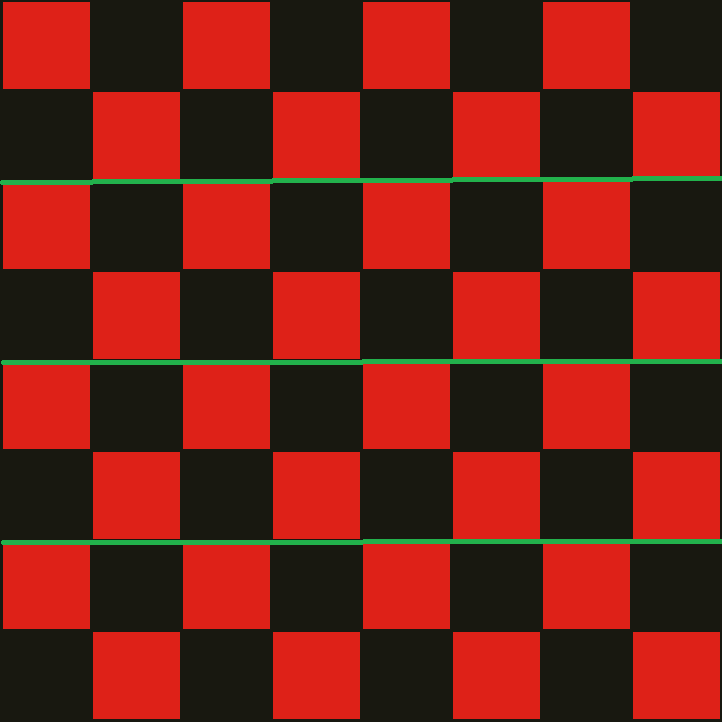
\includegraphics[width=33mm]{img/red-black-grid.png}
    \end{figure}
	\item Tại mỗi bước lặp, cập nhật các ô màu \emph{đỏ} trước, sau đó cập nhật các ô màu \emph{đen}.
	\item Các ô cùng màu được cập nhật song song theo \emph{thứ tự hàng}.
	\item \textbf{Nhận xét:} Các ô màu đỏ được cập nhật hoàn toàn dựa vào kết quả ở bước lặp trước (bước $i$), các ô màu đen được cập nhật hoàn toàn dựa vào kết quả ở bước lặp hiện tại (bước $i + 1$).
\end{itemize}
\end{frame}

\section{Công thức phát triển}
\begin{frame}{Công thức phát triển}
\begin{itemize}
    \item Công thức xác suất phát triển
    \begin{equation}
    	p_g((l, m) \in Z) = \frac{(c_{l, m})^{\eta}}{\sum_{(l, m) \in Z}^{} (c_{l, m})^{\eta}}
	\end{equation}
	\item $Z$ là tập các ô lân cận với các ô mà trực khuẩn đang chiếm.
	\item Công thức phát triển
	\begin{equation}
		c_{l, m} = I\{rand(0, 1) < p_g(l, m)\}
	\end{equation}
\end{itemize}
\end{frame}

\section{Song song hoá quá trình phát triển}
\begin{frame}{Song song hoá quá trình phát triển}
\begin{itemize}
	\item Gồm 2 bước: Tính xác suất và phát triển ngẫu nhiên.
	\item \textbf{Nhận xét:} Mỗi bước trên có thể thực hiện song song và thứ tự tính toán không ảnh hưởng đến kết quả cuối cùng.
    \item Sử dụng \emph{thứ tự hàng}, lần lượt tính xác suất song song và cho trực khuẩn phát triển ngẫu nhiên song song.
\end{itemize}
\end{frame}

\section{Sơ đồ luồng thuật toán}
\begin{frame}{Sơ đồ luồng thuật toán}
\begin{itemize}
	\item Sơ đồ luồng thuật toán
    \begin{figure}[H]
        \centering
        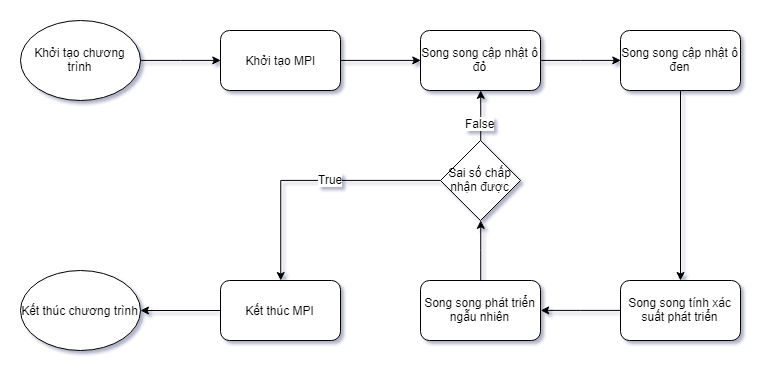
\includegraphics[width=77mm]{img/algo-flowchart.png}
    \end{figure}
\end{itemize}
\end{frame}

\section{Kết quả mô phỏng}
\begin{frame}[allowframebreaks]{Kết quả mô phỏng}
\begin{itemize}
	\item $N = 40, \eta = 1, i = 100$
    \begin{figure}[H]
        \centering
        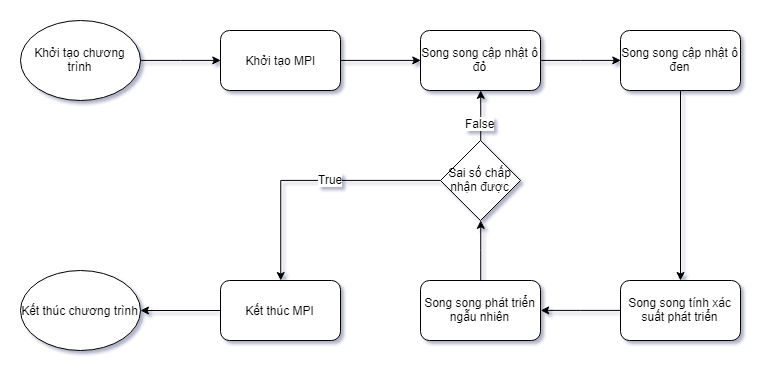
\includegraphics[width=77mm]{img/algo-flowchart.png}
    \end{figure}
\end{itemize}
\break
\begin{itemize}
    \item $N = 40, \eta = 1, i = 200$
    \begin{figure}[H]
        \centering
        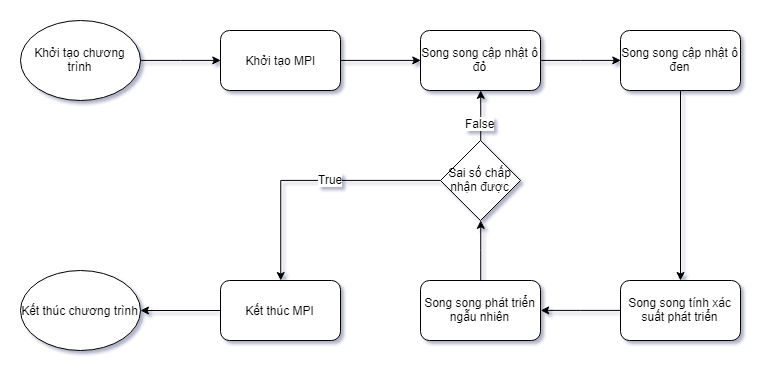
\includegraphics[width=77mm]{img/algo-flowchart.png}
    \end{figure}
\end{itemize}
\break
\begin{itemize}
    \item $N = 40, \eta = 1, i = 500$
    \begin{figure}[H]
        \centering
        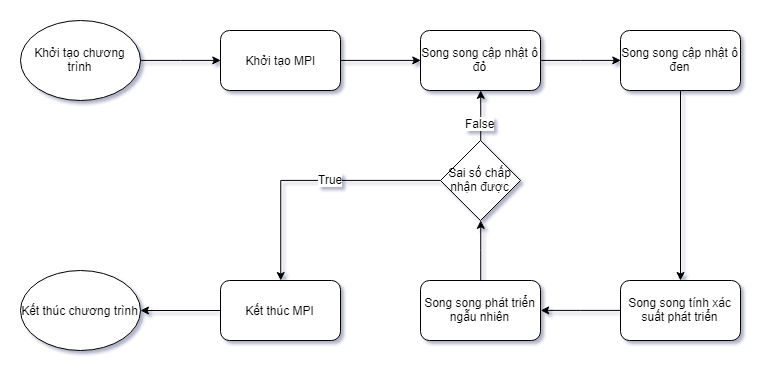
\includegraphics[width=77mm]{img/algo-flowchart.png}
    \end{figure}
\end{itemize}
\break
\begin{itemize}
    \item $N = 40, \eta = 1, i = 1000$
    \begin{figure}[H]
        \centering
        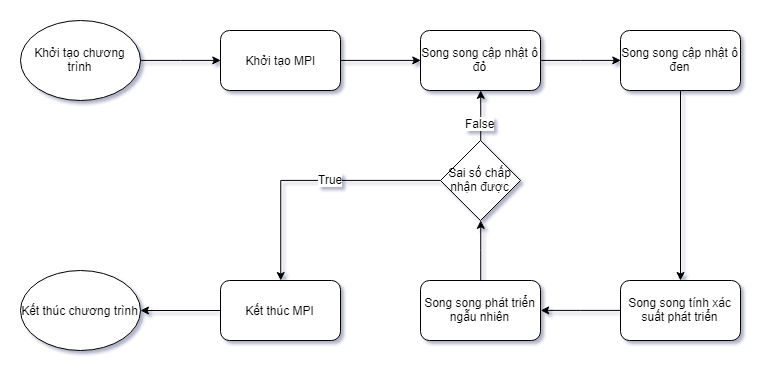
\includegraphics[width=77mm]{img/algo-flowchart.png}
    \end{figure}
\end{itemize}
\break
\begin{itemize}
    \item $N = 40, \eta = 2, i = 100$
    \begin{figure}[H]
        \centering
        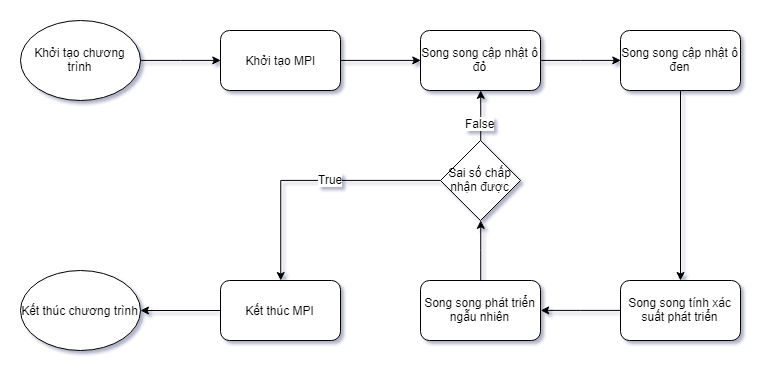
\includegraphics[width=77mm]{img/algo-flowchart.png}
    \end{figure}
\end{itemize}
\break
\begin{itemize}
    \item $N = 40, \eta = 2, i = 200$
    \begin{figure}[H]
        \centering
        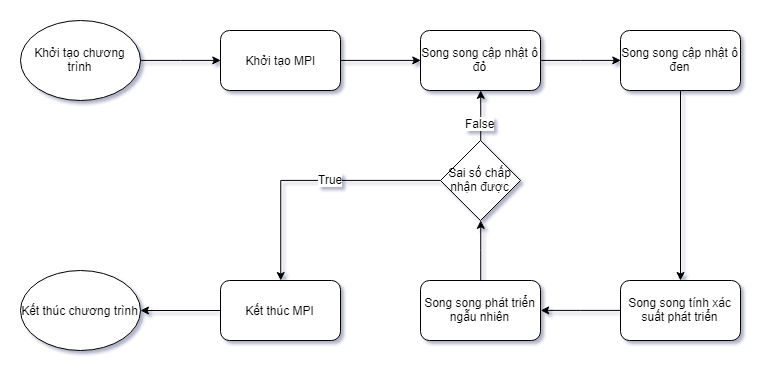
\includegraphics[width=77mm]{img/algo-flowchart.png}
    \end{figure}
\end{itemize}
\break
\begin{itemize}
    \item $N = 40, \eta = 2, i = 500$
    \begin{figure}[H]
        \centering
        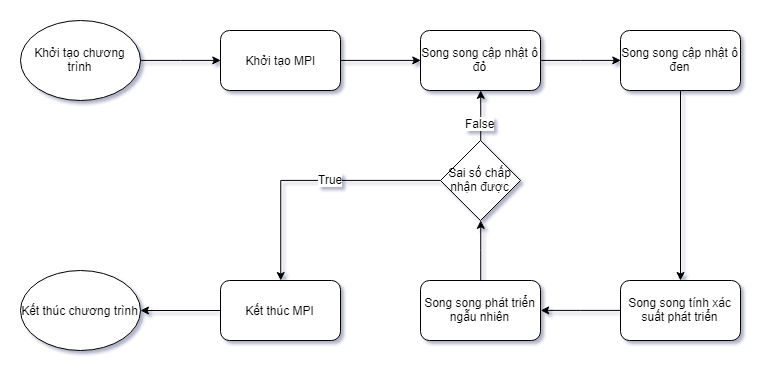
\includegraphics[width=77mm]{img/algo-flowchart.png}
    \end{figure}
\end{itemize}
\break
\begin{itemize}
    \item $N = 40, \eta = 2, i = 1000$
    \begin{figure}[H]
        \centering
        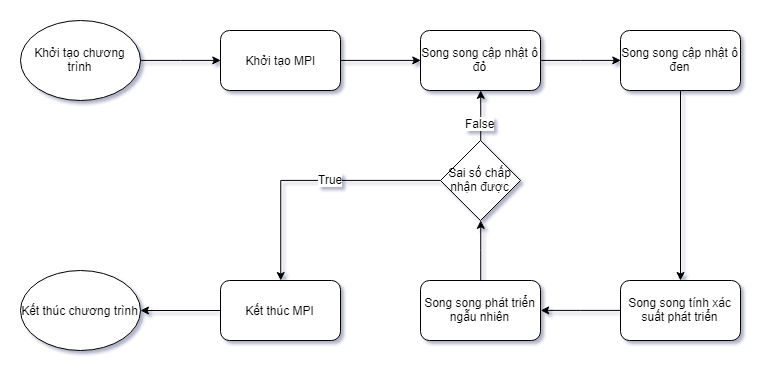
\includegraphics[width=77mm]{img/algo-flowchart.png}
    \end{figure}
\end{itemize}
\break
\begin{itemize}
    \item $N = 40, \eta = 0.5, i = 100$
    \begin{figure}[H]
        \centering
        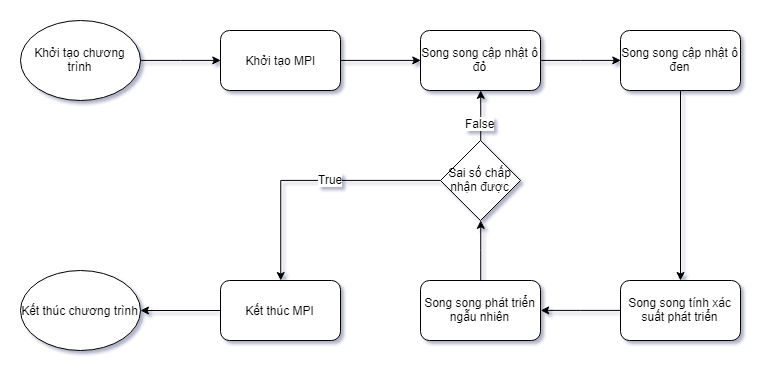
\includegraphics[width=77mm]{img/algo-flowchart.png}
    \end{figure}
\end{itemize}
\break
\begin{itemize}
    \item $N = 40, \eta = 0.5, i = 200$
    \begin{figure}[H]
        \centering
        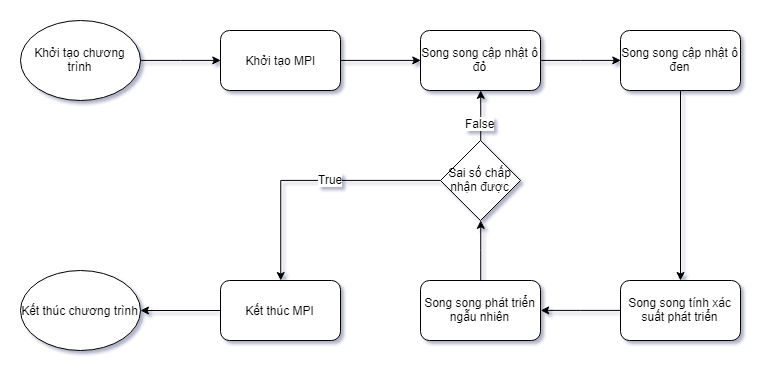
\includegraphics[width=77mm]{img/algo-flowchart.png}
    \end{figure}
\end{itemize}
\break
\begin{itemize}
    \item $N = 40, \eta = 0.5, i = 500$
    \begin{figure}[H]
        \centering
        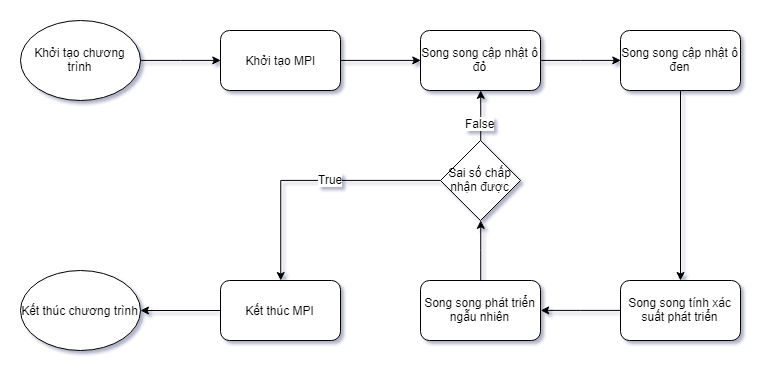
\includegraphics[width=77mm]{img/algo-flowchart.png}
    \end{figure}
\end{itemize}
\break
\begin{itemize}
    \item $N = 40, \eta = 0.5, i = 1000$
    \begin{figure}[H]
        \centering
        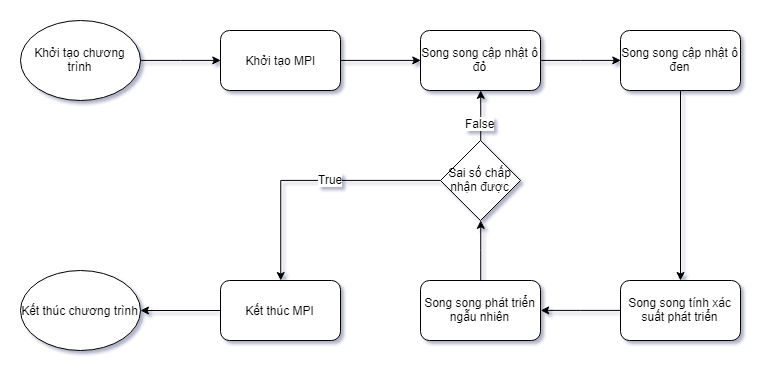
\includegraphics[width=77mm]{img/algo-flowchart.png}
    \end{figure}
\end{itemize}
\end{frame}

\begin{frame}{Cảm ơn}
    \large{Cảm ơn thầy và các bạn đã chú ý lắng nghe.}
\end{frame}

\begin{frame}
\titlepage 
\end{frame}


\end{document}